\section{splittable Task}

In the previous chapter we proposed an analytical model for execution time of a balanced parallel for loop in terems of the grain size, and based on this model, we offered an approach to find the range of grain size to achieve minimum exection time. The parameters of the propoesd model is identified through a benchmark and is exposed to the Blaze library to be used to predict the range of grain size for minimum excution time of a problem with a size that would be revealed at run-time. So the proposed solution is a combination of a compile-time and run-time solution to improve the performnace.
  
In this chapter we take another direction to tackle the problem of improving the performance through a run-time adaptive solution.

In \cite{thoman2013adaptive}, the authors offer a combination of compile-time and run-time solution for adaptive control of task granulartity. 

Lazy scheduling, \cite{tzannes2014lazy}

Splittable tasks are tasks that could be partitioned into smaller tasks, when sufficient parallelism is available\cite{prell2016embracing}. 

Utilizing splittable tasks is an approach to avoid creating large overhead of work stealing. 
Based on work stealing, in order to decrease the overhead of work stealing. 

\cite{aguilar2019line}


\subsection{Implementation}
For a for-loop with the range of $[a,b)$ one splittable task containg all the iterations from $a$ to $b-1$ would be created. Depending on the splitting strateg when a certain condition is met this task would be splitted into two parts, one containg iterations in the range of $[a,c)$ and the other part from $[c,b)$, where $c$ is the split point.   

 
\subsection{Splitting Strategies}
The splttable task could be splitted either based on total number of cores available, or number of idle cores at the time of split. 

\subsubsection{Splitting based on total number of cores}

\subsubsection{Splitting based on number of idle cores}

\subsection{Results}

\subsubsection{For-loop Benchmark}

\begin{figure}[H]
	\centering
	\subfloat[]
	{\centering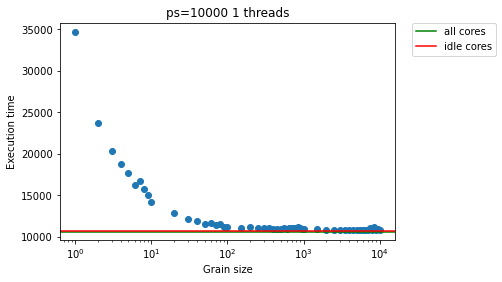
\includegraphics[scale=.35]{images/hpx_for_loop/splittable/all_idle_cores/marvin_10000_1.png}	
		\label{fig66:a}}
	\subfloat[]
	{\centering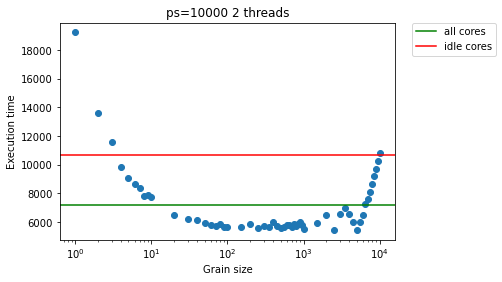
\includegraphics[scale=.35]{images/hpx_for_loop/splittable/all_idle_cores/marvin_10000_2.png}	
		\label{fig66:b}}\hfill
	\subfloat[]
	{\centering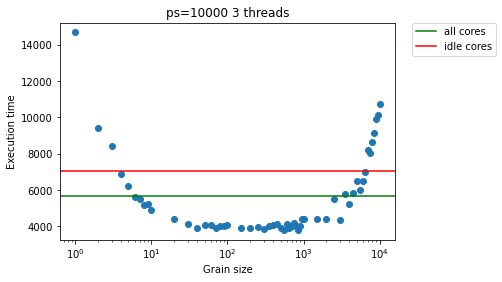
\includegraphics[scale=.35]{images/hpx_for_loop/splittable/all_idle_cores/marvin_10000_3.png}	
		\label{fig66:c}}
	\subfloat[]
	{\centering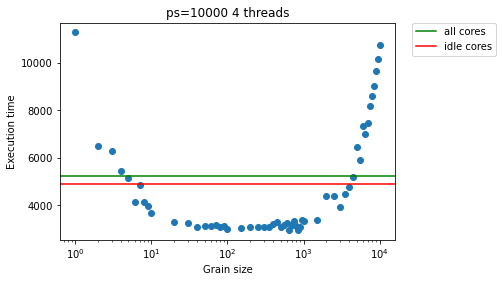
\includegraphics[scale=.35]{images/hpx_for_loop/splittable/all_idle_cores/marvin_10000_4.png}	
		\label{fig66:d}}\hfill
	\subfloat[]
	{\centering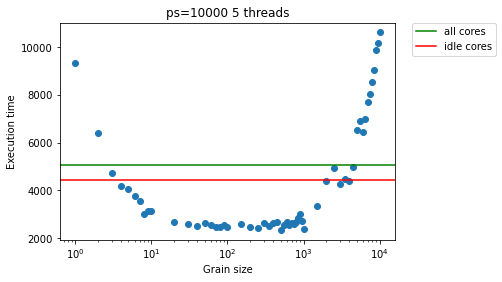
\includegraphics[scale=.35]{images/hpx_for_loop/splittable/all_idle_cores/marvin_10000_5.png}	
		\label{fig66:e}}
	\subfloat[]
	{\centering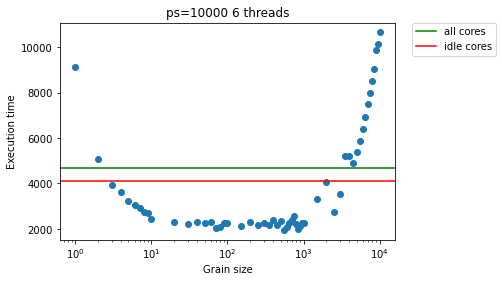
\includegraphics[scale=.35]{images/hpx_for_loop/splittable/all_idle_cores/marvin_10000_6.png}	
		\label{fig66:f}}\hfill
	\subfloat[]
	{\centering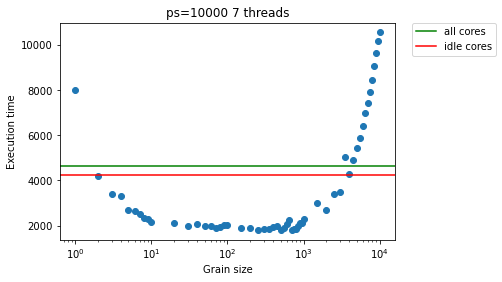
\includegraphics[scale=.35]{images/hpx_for_loop/splittable/all_idle_cores/marvin_10000_7.png}	
		\label{fig66:g}}
	\subfloat[]
	{\centering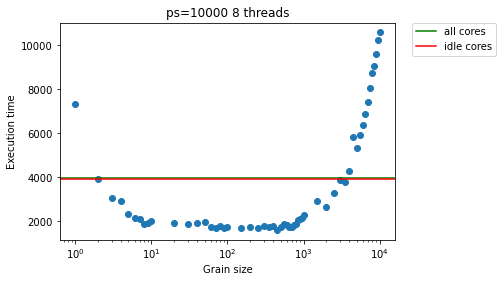
\includegraphics[scale=.35]{images/hpx_for_loop/splittable/all_idle_cores/marvin_10000_8.png}	
		\label{fig66:h}}\hfill
	\caption{The results of running the hpx for loop using splittable tasks with all-cores and idle-cores split types compared with different grain sizes, for $problem\_size=10000$, for (a) 1 core, (b) 2 cores, (c) 3 cores, (d) 4 cores, (e) 5 cores, (f) 6 cores, (g) 7 cores, (h) 8 cores. The unit for execution time is microseconds.}
	\label{fig66}	
\end{figure}

\subsubsection{Blazemark}